% !Mode::"TeX:UTF-8"
\documentclass[twocolumn,landscape,UTF8]{ctexart}
\usepackage{lastpage}
%\usepackage{times} %use the Times New Roman fonts
\usepackage{color}
%\usepackage{placeins}
\usepackage{ulem}
\usepackage{titlesec}
\usepackage{graphicx}
\usepackage{colortbl}
\usepackage{listings}
\usepackage{makecell}
\usepackage{indentfirst}
\usepackage{fancyhdr}
\usepackage{setspace} % 行间距
\usepackage{bm}%\boldsymbol 粗体
% 数学
\usepackage{amsmath,amsfonts,amsmath,amssymb,times}
\usepackage{txfonts}
\usepackage{enumerate}% 编号
\usepackage{tikz,pgfplots} %绘图
\usepackage{tkz-euclide,pgfplots}
\usetikzlibrary{automata,positioning}
%\usepackage[paperwidth=18.4cm,paperheight=26cm,top=1.5cm,bottom=2cm,right=2cm]{geometry} % 单页
\usepackage[paperwidth=36.8cm,paperheight=26cm,top=2.5cm,bottom=2cm,right=2cm]{geometry}
\lstset{language=C,keywordstyle=\color{red},showstringspaces=false,rulesepcolor=\color{green}}
\oddsidemargin=0.5cm   %奇数页页边距
\evensidemargin=0.5cm %偶数页页边距
%\textwidth=14.5cm        %文本的宽度 单页
\textwidth=30cm        %文本的宽度 单页

\newsavebox{\zdx}%装订线

\newcommand{\putzdx}{\marginpar{
		\parbox{1cm}{\vspace{-1.6cm}
			\rotatebox[origin=c]{90}{
				\usebox{\zdx}
		}}
}}

\newcommand{\blank}{\uline{\textcolor{white}{a}\ \textcolor{white}{a}\ \textcolor{white}{a}\ \textcolor{white}{a}\ \textcolor{white}{a}\ \textcolor{white}{a}\ \textcolor{white}{a}\ \textcolor{white}{a}\ \textcolor{white}{a}\ \textcolor{white}{a}\ \textcolor{white}{a}}}

\newcommand{\me}{\mathrm{e}}  %定义 对数常数e,虚数符号i,j以及微分算子d为直立体。
\newcommand{\mi}{\mathrm{i}}
\newcommand{\mj}{\mathrm{j}}
\newcommand{\dif}{\mathrm{d}}
\newcommand{\bs}{\boldsymbol}%数学黑体
\newcommand{\ds}{\displaystyle}
%通常我们使用的分数线是系统自己定义的分数线,即分数线的长度的预设值是分子或分母所占的最大宽度,如何让分数线的长度变长成,我们%可以在分子分母添加间隔来实现。如中文分式的命令可以定义为:
%\newcommand{\chfrac[2]}{\cfrac{\;#1\;}{\;#2\;}}
%\frac{1}{2} \qquad \chfrac{1}{2}

%选择题
\newcommand{\fourch}[4]{\\\begin{tabular}{*{4}{@{}p{3.5cm}}}(A)~#1 & (B)~#2 & (C)~#3 & (D)~#4\end{tabular}} % 四行
\newcommand{\twoch}[4]{\\\begin{tabular}{*{2}{@{}p{7cm}}}(A)~#1 & (B)~#2\end{tabular}\\\begin{tabular}{*{2}{@{}p{7cm}}}(C)~#3 &
		(D)~#4\end{tabular}}  %两行
\newcommand{\onech}[4]{\\(A)~#1 \\ (B)~#2 \\ (C)~#3 \\ (D)~#4}  % 一行

\renewcommand{\headrulewidth}{0pt}
\pagestyle{fancy}
\begin{document} % 在begin前面加了一个空格以免出现显示错误,编译时应该去掉
\fancyhf{}
\fancyfoot[CO,CE]{\vspace*{1mm}第\,\thepage\,页 , 共 ~\pageref{LastPage} 页}
\sbox{\zdx}
{\parbox{27cm}{\centering
	座位号~\underline{\makebox[34mm][c]{}}~ 班~级\underline{\makebox[34mm][c]{}}~\CJKfamily{song} 学~号\underline{\makebox[44mm][c]{}}~\CJKfamily{song} 姓~名\underline{\makebox[34mm][c]{}} ~\\
	\vspace{3mm}
请在所附答题纸上空出密封位置。并填写试卷序号、班级、学号和 姓名\\
%答题时学号
\vspace{1mm}
\dotfill{} 密\dotfill{}封\dotfill{}线\dotfill{} \\
	}}
	\reversemarginpar
	
\begin{spacing}{1.25}
	\begin{center}
\begin{LARGE}
文华学院~\underline{~2018 }\,年第\,\underline{~2018--2019秋季~}\,学期\\
\underline{合同法}\,期末考试试卷\\
\end{LARGE}
(闭卷笔试\ \ 90 分钟)\\
	\vspace{0.5cm}
\begin{tabular}{|m{0.03\textwidth}|*{8}{m{0.035\textwidth}|}p{0.04\textwidth}|}
	\hline
\centering  题~号 & \centering 一 & \centering 二 & \centering 三 & \centering 四& \centering 五 & \centering 六 & \centering 七 % & \centering 八 & \centering 九 & \centering 十
& \centering 总~分 & \makecell{阅卷\\教师} \rule{0pt}{3mm} \\
	\hline
	\centering 分~数 &  &  &  &  &  &  &  &  &  %&  &
	\rule{0pt}{8mm} \\\hline
				% \centering 计 &  &  &  &  &  &  &  &  &  &  & \\
				% \centering 分 &  &  &  &  &  &  &  &  &  &  & \\
				% \centering 人 &  &  &  &  &  &  &  &  &  &  & \\  \hline
\end{tabular}
\end{center}
\end{spacing}
\vspace{-0.5cm}
\setlength{\marginparsep}{1.7cm}
\putzdx %%装订线--奇页数
\vspace{1cm}
	\begin{spacing}{1.3}
		
		\section*{\hspace{5cm} 一、单项选择题~(每题~2 分,共~20 题,40分)}
		\vspace{-2cm}
		\begin{tabular}{|p{0.05\textwidth}|p{0.05\textwidth}|}
			\hline
			% after \\: \hline or \cline{col1-col2} \cline{col3-col4} ...
			\centering 阅卷人& \\
			\hline
			\centering 得~~分 &  \\
			\hline
		\end{tabular}
		
\begin{enumerate}\setcounter{enumi}{0}

\item 我国民法的调整对象是(~~~~~)
\onech{一切横向经济关系}{法定范围的财产关系和人身关系}{平等主体间的财产关系和人身关系}{平等主体间的人身关系和完全没有国家参与的财产关系}
\item 某媒体未征得艾滋病孤儿小明的同意,发表了一首关于小明的报道,将其真实姓名、照片和患病经历公之于众。报道发表后,隐去真实身份开始正常生活的小明再次受到歧视和排斥,下列哪选项是正确的?(~~~~~)
\twoch{该媒体的行为不构成侵权}{该媒体侵犯了小明的健康权}{该媒体侵犯了小明的姓名权}{该媒体侵犯了小明的隐私权}
\item 幼儿同的小亮和小明在课向打架,在场的班主任王某未予制止。小明戳伤小亮左眼,致其失明。下列哪一选项是正确的?(~~~~~)
\onech{幼儿园未尽职责范围内的管理、保护义务。应当承担与其过错相应的财产责任。}{幼儿园与小明的父母均有过错,应当由幼儿园与小明的父母承担连带赔偿责任。}{父母的监护责任已经转移到幼儿园,应由幼儿园承担赔偿责任。}{王某存在过错,应当由王某承担赔偿责任。}
\item 就我国民事立法中确立的基本原则,下列说法正确的是(~~~~~)
\onech{《合同法》确立公平、等价有偿原则}{《物权法》确立物权法定,一物一权、公示公信原则}{《合同法》确立合同履行中的情势变更原则}{自愿,公平、等价有偿、诚实信用原则在《民法总则》中得以确立}
\item 下列关于代表和代理的说法中正确的是(~~~~~)
\onech{法定代表人的代表职权源于法人的授权}{公司做出的撤销法定代表人的决定自登记公告之日起生效}{委托书授权不明的,被代理人应当向第三人承担民事责任,代理人负连带责任}{民法通则)明确规定代理人代理行为的法律后果属于被代理人}
\item 甲购买乙的房屋一套,已经付款一半,双方约定余款待房屋办理过户登记手续之后付清,后来房屋升值。乙反悔,要求解除合同,甲不同意要求乙继续履行合同,转移房屋所有权,下列选项正确的是(~~~~~)
\onech{合同尚末生效,乙应当返还受领的价款并承担缔约过失责任}{合同无效。因为房屋过户手续尚未办理}{合同有效。乙应继续履行合同}{该案中房屋过户手续已经完成,而合同确实存在无效原因,甲仍然可以基于所有权登记主张对房屋的所有权,并对抗乙确认合同无效的诉权}


\end{enumerate}
\newpage
\section*{\hspace{4.5cm} 二、案例分析题 (15分)}
\vspace{-1cm}
\begin{tabular}{|p{0.05\textwidth}|p{0.05\textwidth}|}
\hline
			% after \\: \hline or \cline{col1-col2} \cline{col3-col4} ...
\centering 阅卷人& \\
\hline
\centering 得~~分 &  \\
	\hline
\end{tabular}
\begin{enumerate}\setcounter{enumi}{5}
	\itshape 2018年2月10日,甲公司与乙公司签订了一份购买乙公司生产的1000台A型微波护的合同,约定由乙公司3月10日前办理托运手续。货到付款。乙公司如期办理了托运手比、续,但装货时多装了50台B型微波炉。

	甲公司于3月13日与丙公司签订合同。将处于运输途中的前述合同项下1000台A型微被护转卖给丙公司,约定货物质量检验期为货到后10天内。3月15日,上述货物在运输途中突遇山洪暴发。致使100台A型微被护受损报废。3
	
	月20日货到丙公司。4月15日内公司以部分货物质量不符合约定为由拒付货款,并要求退费。
	
	\normalfont
	问题:
	(1)如乙公司在办理完托运手续后即请求甲公司付款,甲公司应否付款?为什么? (3分)

	(2)乙公司办理完托运手续后,贷物的所有权归谁?为什么? (3分)

	(3)对因山洪暴发报废的100台微波护,应当由谁承担风险损失?为什么?(3分)

	(4)对于乙公司多装的50台B型微波炉。应当如何处理?为什么? (3分)

	(5)丙公司能否拒货款成和要求退费?为什么? (3分)
\end{enumerate}

\vspace{2cm}
\section*{\hspace{5cm} 三、填空题~(每题~3 分, 共~ 15 分)}
\vspace{-1cm}

\begin{tabular}{|p{0.05\textwidth}|p{0.05\textwidth}|}
			\hline
			% after \\: \hline or \cline{col1-col2} \cline{col3-col4} ...
			\centering 阅卷人& \\
			\hline
			\centering 得~~分 &  \\
			\hline
		\end{tabular}
		\begin{enumerate}\setcounter{enumi}{10}
			\item ~$\lim\limits_{x\rightarrow \infty}(1-x)^{\frac{\,1\,}{x}}=$ ~\underline{~~~$\me^{-1}$~~~}.
			
			\item 设~$z = u^2\ln v$ , 而~$u= \dfrac{x}{y}, v = x-y$ , 则~$\dfrac{\partial z}{\partial x}= $~\underline{~~$\dfrac{2x}{y^2}\ln(x-y)+\dfrac{x^2}{y^2(x-y)}$~~}.
			
			\item 函数~$f(x,y) = x\me^y$ 在点~$(1,0)$ 处的梯度为~$\nabla f = $~\underline{~~~~$(1,2)$~~~~~}.
			\item 把二次积分~$\displaystyle{\int_0^1 \dif x \int_0^{\sqrt{1-x^2}} f(x,y) \dif y}$ 化为极坐标形式的二次积分为\\
			~\underline{~~~$\displaystyle{\int_0^{\pi/2} \dif \theta \int_0^1 f(\rho \cos\theta, \rho\sin\theta)\rho \dif \rho}$~~~~}.
			%\item 设积分区域~$D= \{(x,y)|0\leqslant y \leqslant 1, 0\leqslant x\leqslant y\}$, 则二重积分
			%\vspace{1cm} ~$\ds{\iint_D\me^{-y^2}\dif x \dif y }= $ ~\underline{~~$\dfrac{1}{2}(1-\me^{-1})$~~}.
			
			\item 设幂级数~$\sum\limits_{n=0}^\infty a_nx^n$ 的收敛半径为~$3$, 则幂级~$\sum\limits_{n=0}^\infty a_nx^{2n}$ 的收敛半径为~\underline{~~~~$\sqrt{3}$~~~~~}.
		\end{enumerate}
		
		\newpage
		\putzdx %%装订线--奇页数
		
		\section*{\hspace{5cm} 四、多元函数微分法~(每题~7分, 共~21分)}
		\vspace{-2cm}
		\begin{tabular}{|p{0.05\textwidth}|p{0.05\textwidth}|}
			\hline
			% after \\: \hline or \cline{col1-col2} \cline{col3-col4} ...
			\centering  阅卷人&  \\
			\hline
			\centering 得~~分 &  \\
			\hline
		\end{tabular}
		\begin{enumerate}\setcounter{enumi}{15}
		\item 设~$\bs{a}=(3,4,5),~\bs{b}=(1,-2,3)$, 求~$\bs{a}\cdot\bs{b}$, $\bs{a}$ 在 $ \bs{b}$ 上的投影, ~$\bs{a}\times\bs{b}$.
		\vspace{1cm}
		
		解:~$\bs{a}\cdot\bs{b} = 3-8+15=10$ \dotfill{}(2')
		
		~$(\bs{a})_{\bs{b}} = \dfrac{\bs{a}\cdot\bs{b}}{|\bs{b}|}=\dfrac{10}{\sqrt{14}}$ \dotfill{}(2')
		
		~$\bs{a}\times\bs{b} = \begin{vmatrix}
		\bs{i} & \bs{j} & \bs{k}\\
		3 & 4 & 5\\
		1 & -2 & 3\\
		\end{vmatrix}=(22,-4,-10).$ \dotfill{}(3')
\item  求过点~$A(1,2,-1), B(2,3,0),C(3,3,2)$ 的三角形~$\triangle ABC$ 的面积和它们确定的平面方程.

解:由题设~$\overrightarrow{AB}=(1,1,1),\overrightarrow{AC}=(2,1,3)$, \dotfill{}(2')

故~$\overrightarrow{AB}\times \overrightarrow{AC}=\begin{vmatrix}
\bs{i}&\bs{j} &\bs{k}\\
1&1&1\\
2&1&3\\
\end{vmatrix}=(2,-1,-1)$,

三角形~$\triangle ABC$ 的面积为~$S_{\triangle ABC}=\dfrac{1}{2}\mid\overrightarrow{AB}\times \overrightarrow{AC}\mid=\dfrac{1}{2}\sqrt{6}.$  \dotfill{}(2')

所求平面的方程为~$2(x-2)-(y-3)-z=0$, 即~$2x-y-z-1=0$
 \dotfill{}(3')			

\item 设函数~$z = f(u,v)$ 具有一阶连续偏导数,~$z = f(x^2+y^2,\dfrac{x}{y})$, 求~$\dfrac{\partial z}{\partial x}, \dfrac{\partial z}{\partial y}$, 并写出全微分~$\dif z$.
			
解: $\dfrac{\partial z}{\partial x} = 2xf_1' + \dfrac{1}{y}f_2'$, \dotfill{}(3')
			
$\dfrac{\partial z}{\partial y} = 2y f_1' - \dfrac{x}{y^2}f_2'$, \dotfill{}(3')
			
$\dif z =\dfrac{\partial z}{\partial x}\dif x + \dfrac{\partial z}{\partial y} \dif y\\	=(2xf_1' + \dfrac{1}{y}f_2')\dif x +(2y f_1' - \dfrac{x}{y^2}f_2')\dif y$, \dotfill{}(1')
\end{enumerate}
\vspace{2cm}

\newpage
\section*{\hspace{5cm}五、重积分~(每题~7 分, 共~ 21 分)}
\vspace{-1cm}
\begin{tabular}{|p{0.05\textwidth}|p{0.05\textwidth}|}
\hline
			% after \\: \hline or \cline{col1-col2} \cline{col3-col4} ...
\centering 阅卷人& \\
\hline
\centering 得~~分 &  \\
\hline
\end{tabular}
		
		\begin{enumerate}\setcounter{enumi}{18}
			\item 计算二重积分~$\ds{\iint\limits_{D}\dfrac{\sin x}{x}\dif \sigma}$, 其中~~$D=\{(x,y)\mid 0\leqslant x \leqslant \pi, 0\leqslant y \leqslant \pi x\}$.
			
			解:
			~$\ds{\iint\limits_{D}\dfrac{\sin x}{x}\dif \sigma}= \ds{\int_0^\pi\dfrac{\sin x}{x}\dif x\int_{0}^{\pi x}\dif y}$  \dotfill{}(2')
			
			~$= \ds{\int_0^\pi\dfrac{\sin x}{x}(\pi x- 0)\dif x = \pi\int_0^\pi\sin x\dif x  }$  \dotfill{}(3')
			
			~$=  \pi\Big[-\cos x \Big]_0^\pi = 2\pi $  \dotfill{}(2')
			
			\item 计算二重积分~$\ds{\iint\limits_{D}\me^{x^2+y^2}\dif \sigma}$, 其中~$D=\{(x,y)\Big| x^2+ y^2 \leqslant 25\}$.
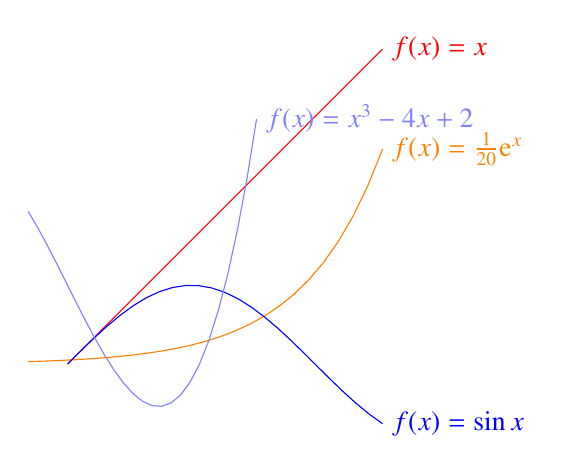
\begin{tikzpicture}[domain=0:4]
\tkzInit[xmax=4.2,ymax=3.2,xmin=-1.2,ymin=-1.2,xstep=1]
%\tkzGrid
\tkzAxeXY
\draw[color=red] plot (\x,\x) node[right] {$f(x)=x$};
\draw[color=orange,domain=-0.5:4] plot (\x,{0.05*exp(\x)}) node[right] {$f(x)=\frac{1}{20}\mathrm e^x$};
\draw[color=blue,domain=0:4] plot (\x,{sin(\x r)}) node[right] {$f(x)=\sin x$};
\draw[color=blue!50,x=1cm,y=0.5cm,domain=-0.5:2.4] plot (\x, {(\x)^3-4*(\x)+2}) node[right] {$f(x)=x^3-4x+2$};
\end{tikzpicture}

			解:~$D: 0\leqslant \theta \leqslant 2\pi, 0\leqslant \rho \leqslant 5$  \dotfill{}(2')
			
			~$\ds{\iint\limits_{D}\me^{x^2+y^2}\dif \sigma}= \ds{\int_0^{2\pi}\dif \theta\int_0^5\me^{\rho^2}\rho\dif \rho}$  \dotfill{}(2')
			
			~$= \ds{2\pi \cdot\Big[\frac{1}{2}\me^{\rho^2}\Big]_0^5 = \pi(\me^{25}-1)} $  \dotfill{}(3')
			
			\vspace{1cm}
			\item 计算三重积分~$\ds{\iiint\limits_{\Omega}z \dif x\dif y\dif z}$, 其中~$\Omega$ 是由~圆锥面~$z = \sqrt{x^2+ y^2}$ 和平面~$z=4$ 围成的闭区域.
			
			解:~$\Omega = \{(x,y,z)\mid x^2 + y^2 \leqslant z^2,0\leqslant z\leqslant 4\}$ \dotfill{}(2')
			
			~$ \ds{\iiint\limits_{\Omega}z \dif x\dif y\dif z =  \int_0^4 z \dif z \iint\limits_{D_z}\dif x\dif y}$ \dotfill{}(3')
			
			~$  = \ds{\int_0^4z\times \pi z^2\dif z= \dfrac{\pi z^4}{4}\Big|_0^4=64\pi}$ \dotfill{}(2')
		\end{enumerate}
		\newpage
		\putzdx %%装订线--奇数页
		\section*{\hspace{5cm} 六、无穷级数~(本题~13 分)}
		\vspace{-2cm}
		\begin{tabular}{|p{0.05\textwidth}|p{0.05\textwidth}|}
			\hline
			% after \\: \hline or \cline{col1-col2} \cline{col3-col4} ...
			\centering  阅卷人& \\
			\hline
			\centering 得~~分 &  \\
			\hline
		\end{tabular}

		\begin{enumerate}\setcounter{enumi}{21}
			\item 求幂级数~$\ds{\sum\limits_{n=1}^\infty\dfrac{(x-1)^n}{n\cdot3^n}} $ 的收敛域与和函数~$s(x)$.
			
			解:令~$t = x-1$, 上述级数变为$\ds{\sum\limits_{n=1}^\infty\dfrac{(x-1)^n}{n\cdot3^n}} $  \dotfill{}(2')
			
			因为 $\rho = \lim\limits_{n\rightarrow\infty}\Big| \dfrac{a_{n+1}}{a_{n}}\Big| = \lim\limits_{n\rightarrow\infty}\dfrac{n\cdot3^n}{(n+1)\cdot3^{n+1}} = \dfrac{1}{3}$, \dotfill{}(2')
			
			所以,收敛半径$R=3 $ 收敛区间~$|t|<3$, 即~$-2<x<4$. \dotfill{}(3')
			
			当~$x = 4$ 时,级数变为~$\sum\limits_{n=1}^\infty\dfrac{1}{n}$ , 这级数发散, 当~$x = -2$ 时,级数变为~$\sum\limits_{n=1}^\infty\dfrac{(-1)^n}{n}$ , 这级数收敛, 原级数的收敛域为~$[-2,4)$.  \dotfill{}(2')
			
			设~$s(x) = \sum\limits_{n=1}^\infty\dfrac{(x-1)^n}{n\cdot3^n}$ , 则
			
			$s'(x) = \sum\limits_{n=1}^\infty\left(\dfrac{(x-1)^n}{n\cdot3^n}\right)' = \sum\limits_{n=1}^\infty\dfrac{(x-1)^{n-1}}{3^n} = \dfrac{\frac{1}{3}}{1-\frac{x-1}{3}}=\dfrac{1}{4-x}$
			
			$s(1) = 0$, $s(x) = s(1)+\ds{\int_1^x s'(t)\dif t = 0 + \int_1^x\dfrac{1}{4-t}\dif t }$
			
			$\ds{ =-\ln(4-t)\Big|_1^x = \ln3-\ln(4-x),-2\leqslant x<4.}$ \dotfill{}(4')
		\end{enumerate}
	
	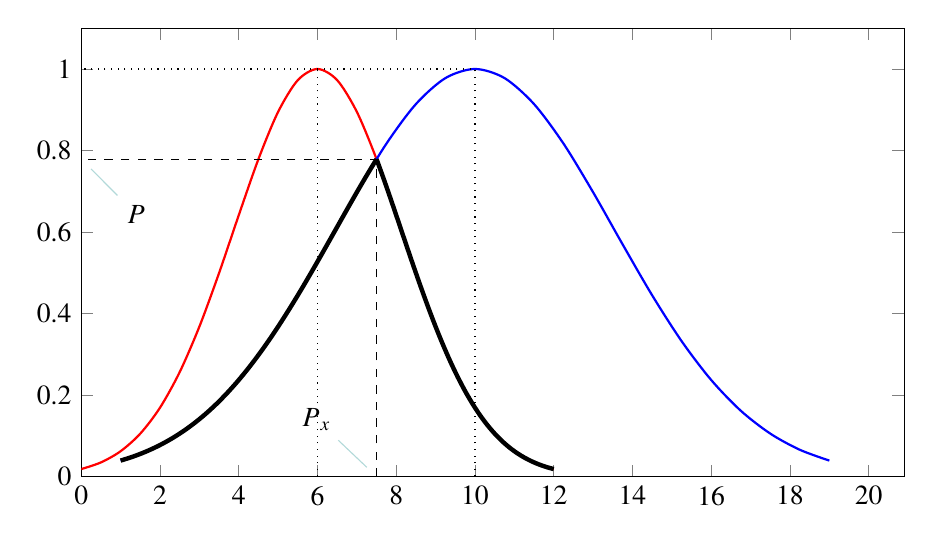
\begin{tikzpicture}
	\begin{axis}[x=.5cm,xmin=0,ymin=0]
	\addplot[mark=none,smooth,red,thick] expression[domain=0:12]{exp(((x-6)^2)/(-9))};
	\addplot[mark=none,smooth,blue,thick] expression[domain=1:19]{exp(((x-10)^2)/(-25))};
	\addplot[mark=none,smooth,ultra thick] expression[domain=7.5:12]{exp(((x-6)^2)/(-9))};
	\addplot[mark=none,smooth,ultra thick] expression[domain=1:7.5]{exp(((x-10)^2)/(-25))};
	\addplot[dotted,mark=none]coordinates{(6,0)(6,1)};
	\addplot[dotted,mark=none]coordinates{(10,0)(10,1)(0,1)};
	\addplot[dashed,mark=none]coordinates{(7.5,0)(7.5,0.7788)(0,0.7788)};
	\node[pin=-45:{$P$}] at (axis cs:0,0.7788) {};
	\node[pin=135:{$P_x$}] at (axis cs:7.5,0) {};
	\end{axis}
	\end{tikzpicture}
	\end{spacing}
\newpage
\begin{tikzpicture}
\begin{axis}
\addplot[color=red]{exp(x)};
\end{axis}
\end{tikzpicture}
%Here ends the furst plot
\hskip 5pt
%Here begins the 3d plot
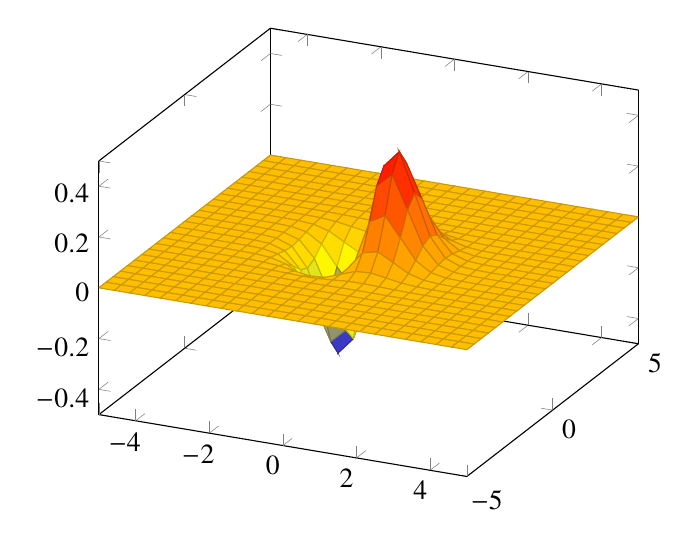
\begin{tikzpicture}
\begin{axis}
\addplot3[
surf,
]
{exp(-x^2-y^2)*x};
\end{axis}
\end{tikzpicture}
文字环绕 文字环绕文字环绕文字环绕文字环绕文字环绕文字环绕文字环绕
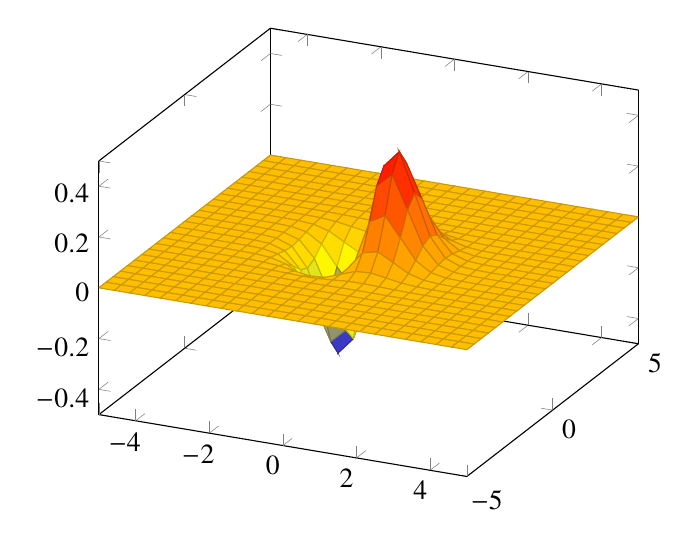
\begin{tikzpicture}
\begin{axis}
\addplot3[
surf,
]
{exp(-x^2-y^2)*x};
\end{axis}
\end{tikzpicture}

	\clearpage
	
\end{document}
